\documentclass[11pt]{article}

\usepackage{deauthor,times,graphicx}
\graphicspath{{submissions/grade-sql-chandra/figs}}
%\usepackage[hidelinks]{hyperref}
\usepackage{hyperref} 

%%%%%%%%%%%%%%%%%%%%%%%%%%%%%%%%%%%%%
\newcommand{\smalltt}[1]{{{\texttt{#1}}}}
\newcommand{\paras}[1]{\noindent\textit{#1}:}
\newcommand{\tabsql}{\hspace*{3mm}}
%%%%%%%%%%%%%%%%%%%%%%%%%%%%%%%%%%%%%

\newcommand\blfootnote[1]{%
  \begin{NoHyper}%
  \renewcommand\thefootnote{}\footnote{#1}%
  \addtocounter{footnote}{-1}%
  \end{NoHyper}%
}

\begin{document}
\title{Automated Grading of SQL Queries}
\author{Bikash Chandra*\blfootnote{Currently at Meta Platforms Inc.} \hspace{1cm} S. Sudarshan \\ IIT Bombay \\ \texttt{\{bikash,sudarsha\}@cse.iitb.ac.in}}
\maketitle

%%%%%%%%%%%%%%%%%%%%%%%%%%%%%%%%%%%%%%%
\begin{abstract}
In a traditional classroom setting, instructors and teaching assistants either grade SQL queries either manually or using fixed datasets. Manual grading is tedious, error-prone and does not scale well for courses with a large number of students or for online courses. Using fixed datasets may miss even common errors and mark incorrect student queries as correct. In this article, we discuss our system XData that, given a set of correct queries, can automatically evaluate the correctness of SQL queries using datasets designed to catch errors in the given correct queries. If a student query is found to be incorrect, XData can even assign grades to the query based on how close they are to a correct query. In our experience, these techniques can be used to grade queries for settings with a large number of students with little human effort and involvement. 
\end{abstract}

\section{Introduction}  
\label{s:intro}
The past decade has observed a surge in the design and deployment of 
decentralized systems. A key reason for this surge is the growing desire in 
the society to have self-governing democratic financial systems that are not 
under the control of a privileged set of entities. A central control often 
translates to a forced trust model with limited provision to support 
transparency and accountability. The adoption of Blockchain, for example, 
is a by-product of the ability to break away from the forced-central control 
in a trust-worthy fashion~\cite{blockchain-book}. The emerging blockchain 
platforms facilitate a reliable execution of any digital contracts 
(i.e., transactions) in a decentralized manner despite the existence of malicious 
actors. At the core of any blockchain platform is a Byzantine 
fault-tolerant (\BFT{}) consensus protocol and a tamper-proof replicated 
ledger~\cite{bedrock,blockchain-book,scalable-ledger}. The \BFT{} 
protocol helps to achieve {\em consensus} on the order of incoming client 
requests among all the replicas, while the ledger logs this agreement. 

Traditional \BFT{} protocols expect a {\em permissioned} system where the 
identities of all the replicas (i.e., participants) are known prior to any 
consensus as they rely on having a verifiable voting right in a democratic 
setting. These protocols rely on a {\em communication-oriented} consensus 
model, where all the participants exchange endorsements across multiple 
rounds before they can reach a decision~\cite{sharper,pbftj,ahl,poe,rcc,geobft,flexitrust,ringbft,mirbft,basil,hotstuff}.
In these protocols, a system of $\n{}$ replicas can reach a common decision 
if at most $\f{}$ of them are malicious, such that $\n{} \ge 3\f{}+1$. 
The $\n{}$ parties are said to reach a decision when at least a majority 
of honest parties agrees to that decision. This decision is logged by 
requiring all the agreeing parties to {\em sign} the decision. Hence, the 
reached decision is considered {\em tamper-proof} because it has support 
of a majority of honest participants.

Despite being around for more than two decades, traditional \BFT{} protocols 
did not see any major practical applications until the introduction of 
blockchain technology. We attribute {\em two} key factors for this lack of 
adoption. (i) To ensure that the malicious participants do not spawn multiple 
identities, these \BFT{} protocols need an authority (i.e., {\em a forced 
trust gateway}) to verify and register every participant to verify every 
vote~\cite{sybil-attack}; some participants may find this intrusive if they 
do not want to reveal their personal information. (ii) To overwrite the ledger, 
malicious participants just require access to the private keys of honest 
participants. In a sense, the proof of the validity of the ledger is not 
self-contained, and it operates on the assumption that the private-keys 
are kept safe externally indefinitely.

To resolve these challenges, initial blockchain platforms such as 
Bitcoin~\cite{bitcoin} and Ethereum~\cite{ether} offer a {\em permissionless} 
model of consensus. These systems employ the {\em Proof-of-Work} (\PoW{}) 
protocol~\cite{bitcoin,ether}, which follows a {\em computation-oriented} 
consensus model and requires all the participants to compete with each other 
and try to solve a complex puzzle. Whichever participant solves the puzzle 
first gets to add a new entry ({\em block}) to the ledger. As a result, 
\PoW{} protocol eliminates the three challenges seen by traditional \BFT{} 
protocols. (i) Malicious participants can spawn multiple identities, but what 
actually matters is the available compute power. (ii) Each block includes 
the hash of the previous block; overwriting the ledger requires recomputing 
all the blocks making it computationally infeasible. (iii) Since reaching the 
consensus is based on presenting the proof of work that is embedded on the 
ledger (i.e., self-contained), there is no longer any need for external 
safe-keeping of private keys to sign endorsements.

These properties offered by \PoW{} protocol help blockchain platforms to 
design a {\em decentralized economy}, where any person can participate in the 
consensus process, and the economy has a self-generating currency to monetize 
its participants. Monetizing the participants is necessary as the \PoW{} 
protocol expects the participants to spend their resources to solve a complex 
puzzle. Clients of the Bitcoin platform, create transactions that exchange 
Bitcoins and send them to the participants (miners) in the \PoW{} protocol. 
These miners check if the transaction is valid; the client has sufficient 
Bitcoins to transfer. If the transaction is valid, they run \PoW{} protocol to include 
this transaction in the ledger. The winning miner of \PoW{} gets a portion of 
the client's Bitcoin as {\em fees}, while the mining process (\PoW{}) mints  
new tokens to fund the economy. This new token is transferred to the winning 
miner's account and is recorded as a transaction in the block.

The key challenge with platforms like Bitcoin is their {\em practicality}. 
These platforms have abysmally low throughput in the order of $10$ transactions 
per second in part due to inadequate choice of small block sizes. Furthermore, as 
more miners join the network, the complexity of the puzzle has to be increased. 
For example, the complexity of the current Bitcoin puzzle is so high that the 
miners work in large groups to have any positive probability of creating the 
next winning block~\cite{blockchain-book}. Moreover, as miners are competing 
with each other, it leads to massive wastage of computational resources (energy) 
as only the winning miner's efforts are recorded and rewarded. This results in an unsustainable ecosystem~\cite{badcoin,badbadcoin}.

We observe these challenges in the designs of existing \BFT{} protocols and 
blockchain platforms and envision a \DualChain{} system that learns from these 
models and eliminates their key challenges. Essentially, we aim to establish a 
new research agenda; a new field of hybrid consensus protocols that depart from 
competitive consensus to a collaborative consensus that is both resilient and 
sustainable. Our \DualChain{} architecture takes a step in this direction by 
running two consensuses on each client transaction while ensuring there is no 
increase in the latency observed by the client. Each client request is first 
ordered through a state-of-the-art \BFT{} consensus protocol ({\em commitment}), 
subsequently, this ordered request is engraved into the ledger through the 
\PoW-style consensus ({\em settlement}). Specifically, \DualChain{} causes no 
increase in commitment latency while improving the settlement latency observed 
by existing protocols. Ordering the client transaction through a \BFT{} consensus 
protocol first allows our \DualChain{} system to guarantee the following benefits: 
(i) clients receive low-latency responses, and (ii) \PoW{} participants no longer 
need to compete, resulting in a high-throughput sustainable chain. As a result, 
instead of employing the \PoW{} for consensus, we design a novel protocol that 
allows miners to collaborate. We refer to this paradigm as 
{\em Power-of-Collaboration} (\PoC{}). 

Our \PoC{} protocol splits the complex puzzle into disjoint slices and requires 
each miner to work on a distinct slice. This slice distribution significantly 
reduces the resource wastage and provides each honest miner with a reward 
for each new transaction added to the ledger. As each ledger entry is added 
collaboratively, any malicious entity that wishes to overwrite the ledger 
needs to match the computational power of all the existing miners making it 
practically impossible. These features of our \DualChain{} system make it 
lucrative; its design is the bedrock for a secure and efficient decentralized 
economy.

\section{Using Datasets to Check Correctness}
\label{sec:datagen}
Test data generation in XData is done based on the correct queries provided by the instructor. Unlike fixed datasets that are query agnostic, these datasets are designed to catch errors based on the correct queries provided by the instructor and are hence much better at catching errors. 

\subsection{Common Errors in SQL Queries}
Students make several types of errors when writing SQL queries. Some students may use an inner join when a left outer join was required, others may use a count aggregation when a count distinct was needed. Mutation testing is a well-known approach to check the adequacy of test cases for a program~\cite{mutation}. We use a similar approach for mutation testing of SQL queries.  We consider mutations as (syntactically correct) changes to an SQL query. Errors made by student queries may be seen as mutations of the correct query and the incorrect query is called a non-equivalent mutant of the correct query. A dataset that produces different results on the correct and incorrect queries is said to kill the mutation. 

XData produces multiple datasets. The first dataset is aimed to produce a non-empty result for the query. This dataset itself kills several mutations. For the remaining datasets, XData considers single mutations at a time on the correct query provided by the instructor and generates datasets that are targeted to kill the mutations. Each dataset is marked with a tag to indicate which type of mutations a dataset is designed to catch. Note that a dataset designed to catch one type of mutation may catch other types of mutations as well. 

XData considers a large number of mutations in SQL queries including but not limited to the following.
\begin{itemize}
    \item \textbf{Join type mutation}: A join type mutation involves replacing one of \smalltt{\{INNER, LEFT OUTER, RIGHT OUTER\} JOIN} with another.  Since the same join query may be written using different join orders, XData considers mutations across different join orders. Mutations involving missing or additional join orders are also considered. 
%XData nullifies each join condition separately.

    \item \textbf{Selection predicate mutation}: For selection conditions, XData considers mutations of the relational
operator where any occurrence of one of  \{$=, <>, <, >, \leq, \geq$\} is replaced by another or if the selection condition is missing. XData also considers mutations of selection predicates between \texttt{IS NULL} and \smalltt{NOT IS NULL} and for missing \smalltt{IS NULL}. These predicates may be on integer, floating, text attributes or even aggregates. Mutations involving changing the constant in the selection condition are also considered. 
    \item \textbf{Aggregation mutation}: Aggregations may be either unconstrained (at the root of the query tree) or constrained (having a condition with the aggregate). In both cases, the aggregation function can be mutated among \smalltt{MAX, MIN, SUM, AVG, COUNT} and their \smalltt{DISTINCT} versions. 
    Mutations involving \smalltt{COUNT(attr)} to \smalltt{COUNT(*)}, in case \smalltt{attr} is nullable, are also considered. 
    \item \textbf{Group by attribute mutation}: For queries involving the \smalltt{GROUP BY} clause, XData considers mutations involving additional or missing group by attributes both in the presence and absence of the \smalltt{HAVING} clause. 
    \item \textbf{Like operator mutation}: Like operators are used in SQL to match patterns in text attributes. SQL like operators include \smalltt{LIKE, NOT LIKE, ILIKE and NOT ILIKE}. XData considers mutation of any one SQL like operator to other like operators. XData also considers mutations in the patterns used with the LIKE operator such as replacing as '\%' with '\_' and vice versa or missing '\%' or '\_' in the pattern.
    \item \textbf{Nested subquery mutations}: XData considers mutations between \smalltt{IN} $vs.$ \smalltt{NOT IN}, \smalltt{EXISTS} $vs.$ \smalltt{NOT EXISTS} and \smalltt{ALL} $vs.$ \smalltt{ANY/SOME}. Mutations on the queries in the nested subquery are also considered for test data generation so that errors inside subqueries are also caught. 
    \item \textbf{Set operator mutations}: Set operators are used in compound queries to combine the results of two underlying results. Set operator mutations include changing one of the following operators to another: \smalltt{UNION, UNION ALL, INTERSECT, INTERSECT ALL, EXCEPT, EXCEPT ALL}. Similar to nested subqueries, mutations of the subqueries whose results are input to these set operators are also considered. 
    \item \textbf{Distinct mutation}: Duplicates in the results may be filtered using the \smalltt{DISTINCT} clause. XData considers mutations of a missing or extraneous \smalltt{DISTINCT} clause.
\end{itemize}

\subsection{Test Data Generation to Detect Errors}
For each type of mutation, we design specific conditions that the datasets must satisfy in order to kill such mutations. Let us take the following example query to demonstrate the mutations considered for queries with join and selections and how we generate datasets to kill the mutations.

\smalltt{\tabsql SELECT course.course\_id\\
\tabsql FROM course INNER JOIN takes USING(course\_id)\\
\tabsql WHERE course.credits >= 6}

Some of the mutations that XData would consider and the techniques to kill those are the following. 

\begin{enumerate}
\item \textbf{Join type mutation}: Consider the
mutation from department INNER JOIN course to
department LEFT OUTER JOIN course. In order to
kill this mutation, we need to ensure that there is a
tuple in department relation that does not satisfy the
join condition with any tuple in course relation. The
INNER JOIN query would not output that tuple in
the department relation while the LEFT OUTER
JOIN would.

In general, a join query can be specified in a join order
independent fashion, with many equivalent join orders for a given query. Hence, the number of join type
mutations across all these orders is exponential. From
the join conditions specified in the query, XData
forms equivalence classes of $<$relation, attribute$>$
pairs such that elements in the same equivalence
class need to be assigned the same value to meet
(one or more) join conditions. Using these equivalence
classes, XData generates a linear number of datasets
to kill join type mutations across all join orderings.
If a pair of relations involve multiple join conditions
\item \textbf{Selection Predicate mutation}: For killing mutations for the selection condition A1 relop A2, XData
generates 3 datasets where tuples satisfy the conditions (1) A1 $>$ A2, (2) A1 $<$ A2,
and (3) A1 $=$ A2. These three datasets kill all non-
equivalent mutations from one relop to another relop. These datasets also kill mutations because of missing
selection conditions. 

For the given query example the constraints would be (1) \smalltt{course.credits>6}, (2) \smalltt{course.credits<6} and (3) \smalltt{course.credits=6}. If the student query uses a different operator instead of $>=$ or misses the selection condition one of the three datasets will catch the error.
\end{enumerate}

Details on test data generation for killing other types of mutations are presented in \cite{xdata:vldbj15}. We omit the details here for brevity. 

It is not sufficient for only the conditions for killing mutations to be satisfied when generating the test database. The difference at one level, say the join condition must change the result of the query for the difference to be observed in the query result. For the given example query, consider the join mutation. If all tuples in course have grade less than 6, both the \smalltt{INNER JOIN} and the \smalltt{LEFT OUTER JOIN} would give empty results. Hence, when generating a dataset, XData ensures that the tuple has \smalltt{grade >= 6}. 

In order to generate a dataset, we generate constraints using an SMT solver~\cite{smt}. In XData, we support CVC3~\cite{CVC3}, CVC4~\cite{CVC4} as well as Z3~\cite{z3} as the constraint solvers. We encode text attributes as enumerates types and enumerates types are modeled as subtypes of integers or rationals. A tuple type is created for each relation to represent one row and an array of tuples represents the relation table. We also add other database constraints such as primary key and foreign key constraints, unique attribute constraints as well as domain constraints. The domain constraints ensure that we generate the correct types of values for each column of the database, the values generated are within the range specified by the schema and only nullable columns can have NULL values.



We also note that some mutations may be semantically equivalent to the correct queries and it may not be possible to kill such mutations. For such cases, the constraints for killing the mutations would not be satisfiable and the SMT solver would fail to generate the dataset to kill the mutation.

For the given query, a simplified version of the constraints, to generate the dataset that produces a non-empty result would be as follows (assuming none of the columns are nullable).
\begin{verbatim}
%Data definition
DATATYPE course_id = CS-101 | BIO-301 | CS-312 | PHY-101 END;
credits:TYPE = SUBTYPE (LAMBDA (x: INT): x > 1 AND x < 11);
course_tuple_type:TYPE = [course_id,credits];
course: ARRAY INT OF course_tuple_type;

%Primary key constraints
ASSERT FORALL(i:course_index, j:course_index): 
       course[i].0 = course[j].[0] => course[i].1 = course[j].1

%Foreign key constraints
ASSERT FORALL(i: takes_index):
       EXISTS (j: course_index): takes[i].1 = course[j].0;

%Query conditions
ASSERT course[1].0 = takes[1].1;
ASSERT course[1].1 >= 6;
\end{verbatim}

To support nullable columns, we add additional values (outside the domain of the column) for the datatype that correspond to NULL values and explicitly mark those as NULL values. 
Also, in practice, we found that unfolding the constraints (i.e., specifying the constraints for each tuple instead of FORALL, NOT EXISTS) gives us much better performance~\cite{xdata:icde11}. We decide the number of tuples upfront and assert the constraint on each tuple. 

\subsection{Evaluating Correctness of Student Queries}
The dataset generation for each correct query is done once across all students. Based on the datasets generated, XData compares the results of each student query and each correct query provided by the instructor. If all results of the student query are found to match that of a correct query, the student query passes that correct query.

When an instructor specifies multiple correct queries, XData allows the instructor to specify one of the two options 
\begin{itemize}
    \item The additional queries were added to provide more coverage and better testing and all correct queries are equivalent. The student query will need to pass all correct queries for it to be marked as correct. 
    \item The question test provided by the instructor was ambiguous and there could be multiple interpretations of the correct result. In this case, the student query will be marked correct if it passes any one of the correct queries. 
\end{itemize}

The XData system ensures that student queries are safely executed on a different database using temporary tables to ensure that their queries do not interfere with the main database or that the queries of one evaluation do not interfere with another. 


\section{Edit Based Suggestions For Learning}
\label{sec:edit}
Generating test data using correct queries provided by the instructor works great for finding student queries with errors. However, once the query is found to be incorrect, the student should be awarded partial marks based on the extent of correctness. It is also useful to make suggestions to the students so that can understand the errors in their queries. 

One way to award marks for correctness could have been to use the fraction of datasets (generated by XData) that the student query could pass. This approach turns out to be unfair and could penalize small errors heavily while providing a better score to queries that have more errors. Such examples are shown in \cite{xdata:comad}. Another way to grade student queries would be to just check for the differences between the correct query and the student query. However, this approach may deduct more marks than required as explained below.

\subsection{Approach}


The approach we use instead in XData is to compare the student query to each correct query and make changes or edits to the student query to attempt to make it equivalent to the correct query. After each edit, the student query is compared to the correct query  and the changes are stopped once the student query is equivalent to the correct query. 
Checking for equivalence after each edit could have been done using test data generation but that would be very expensive and grading each student query could take minutes. Other approaches for checking equivalence such as Cosette~\cite{cosette} as well as techniques based on tableau~\cite{tableaux1} work on a limited subset of query constructs and were hence not considered.

Marks are deducted based on the required edits. The edits required are also used to suggest what changes the students should have made to their query to make it correct, thereby providing individualized feedback to each student without any additional human involvement. For each type of query construct being edited, the instructor of the course can specify the weight for that edit. For example, for a query where the instructor is evaluating the student's ability to write aggregations correctly, the instructor may want to deduct more marks for errors in aggregation than for other errors. By default, XData assigns equal weight to each edit being considered.

In general, more than one edit may be needed to make the student query equivalent to the correct query. It is important to note that the order in which the edits are made is also important and that is not sufficient to just compare the query trees of the correct query and the student query to find the changes. One edit to a student query may allow us to rewrite other parts of the query in a different way. As an example consider the following pair of queries from Section~\ref{sec:intro}.
\begin{itemize}
    \item Correct query: \smalltt{SELECT * FROM r INNER JOIN s ON (r.A=s.A) WHERE r.A>10}
    \item Student query: \smalltt{SELECT * FROM r INNER JOIN s ON (r.A=s.B) WHERE s.A>10}
\end{itemize}

There are two differences between the student query and the correct query - the selection condition and the join condition. If the student query is graded just based on these differences, marks corresponding to two edits would be deducted. Even if we grade based on the edits required, if the selection condition is edited first, followed by the join condition 2 edits would be required. On the other hand, if the join condition is edited first and the join condition in the student query is changed to \smalltt{r.A=s.A}, the selection condition in the student query becomes equivalent to that of the correct query. 

\subsection{Query Canonicalization}
The student and correct query may be written in different ways. For example, the correct query may use a selection condition \smalltt{A>5} while the student query may write the condition as \smalltt{NOT(A<=5)}. In order to compare the query structure of the student query to the correct query, we need to make them comparable. The student query and the correct query are made comparable by using canonicalizations. 

XData considers two types of canonicalizations:
\begin{itemize}
    \item \textbf{Syntactic Canonicalization}: This is the pre-processing step to reduce irrelevant syntactic differences. These include attribute disambiguation, replacing \smalltt{NOT, BETWEEN, and WITH} constructs and removing \smalltt{ORDER BY} from subqueries. 
    \item \textbf{Semantic Canonicalization}: In this step, based on the query conditions and the database constraints, the queries are canonicalized semantically. Such canonicalizations include but are not limited to removing distinct clauses based on primary key information and converting outer joins to inner joins based on non-nullable foreign key information. 
\end{itemize}
A detailed list of the canonicalizations is provided in ~\cite{xdata:comad}. Such canonicalization rules are often used in query optimizers. However, the goal of the canonicalizations in XData is to get more standard forms of the query.

XData also flattens the query tree where possible (\smalltt{INNER JOIN, UNION(ALL), INTERSECT(ALL)} as well as predicates involving AND or OR).  For the parsed query tree shown in Figure~\ref{fig:parsedTree},  XData would flatten the tree to the one shown in Figure~\ref{fig:flattenedTree}. The flattened tree children are compared in an ordered way for non-commutative operators such as \smalltt{LEFT OUTER JOIN, EXCEPT(ALL)} and \smalltt{ORDER BY} attribute lists while for commutative operators the order of operands is ignored while matching. 


\begin{figure}
	\centering
	\begin{minipage}{0.40\textwidth}
	\centering
	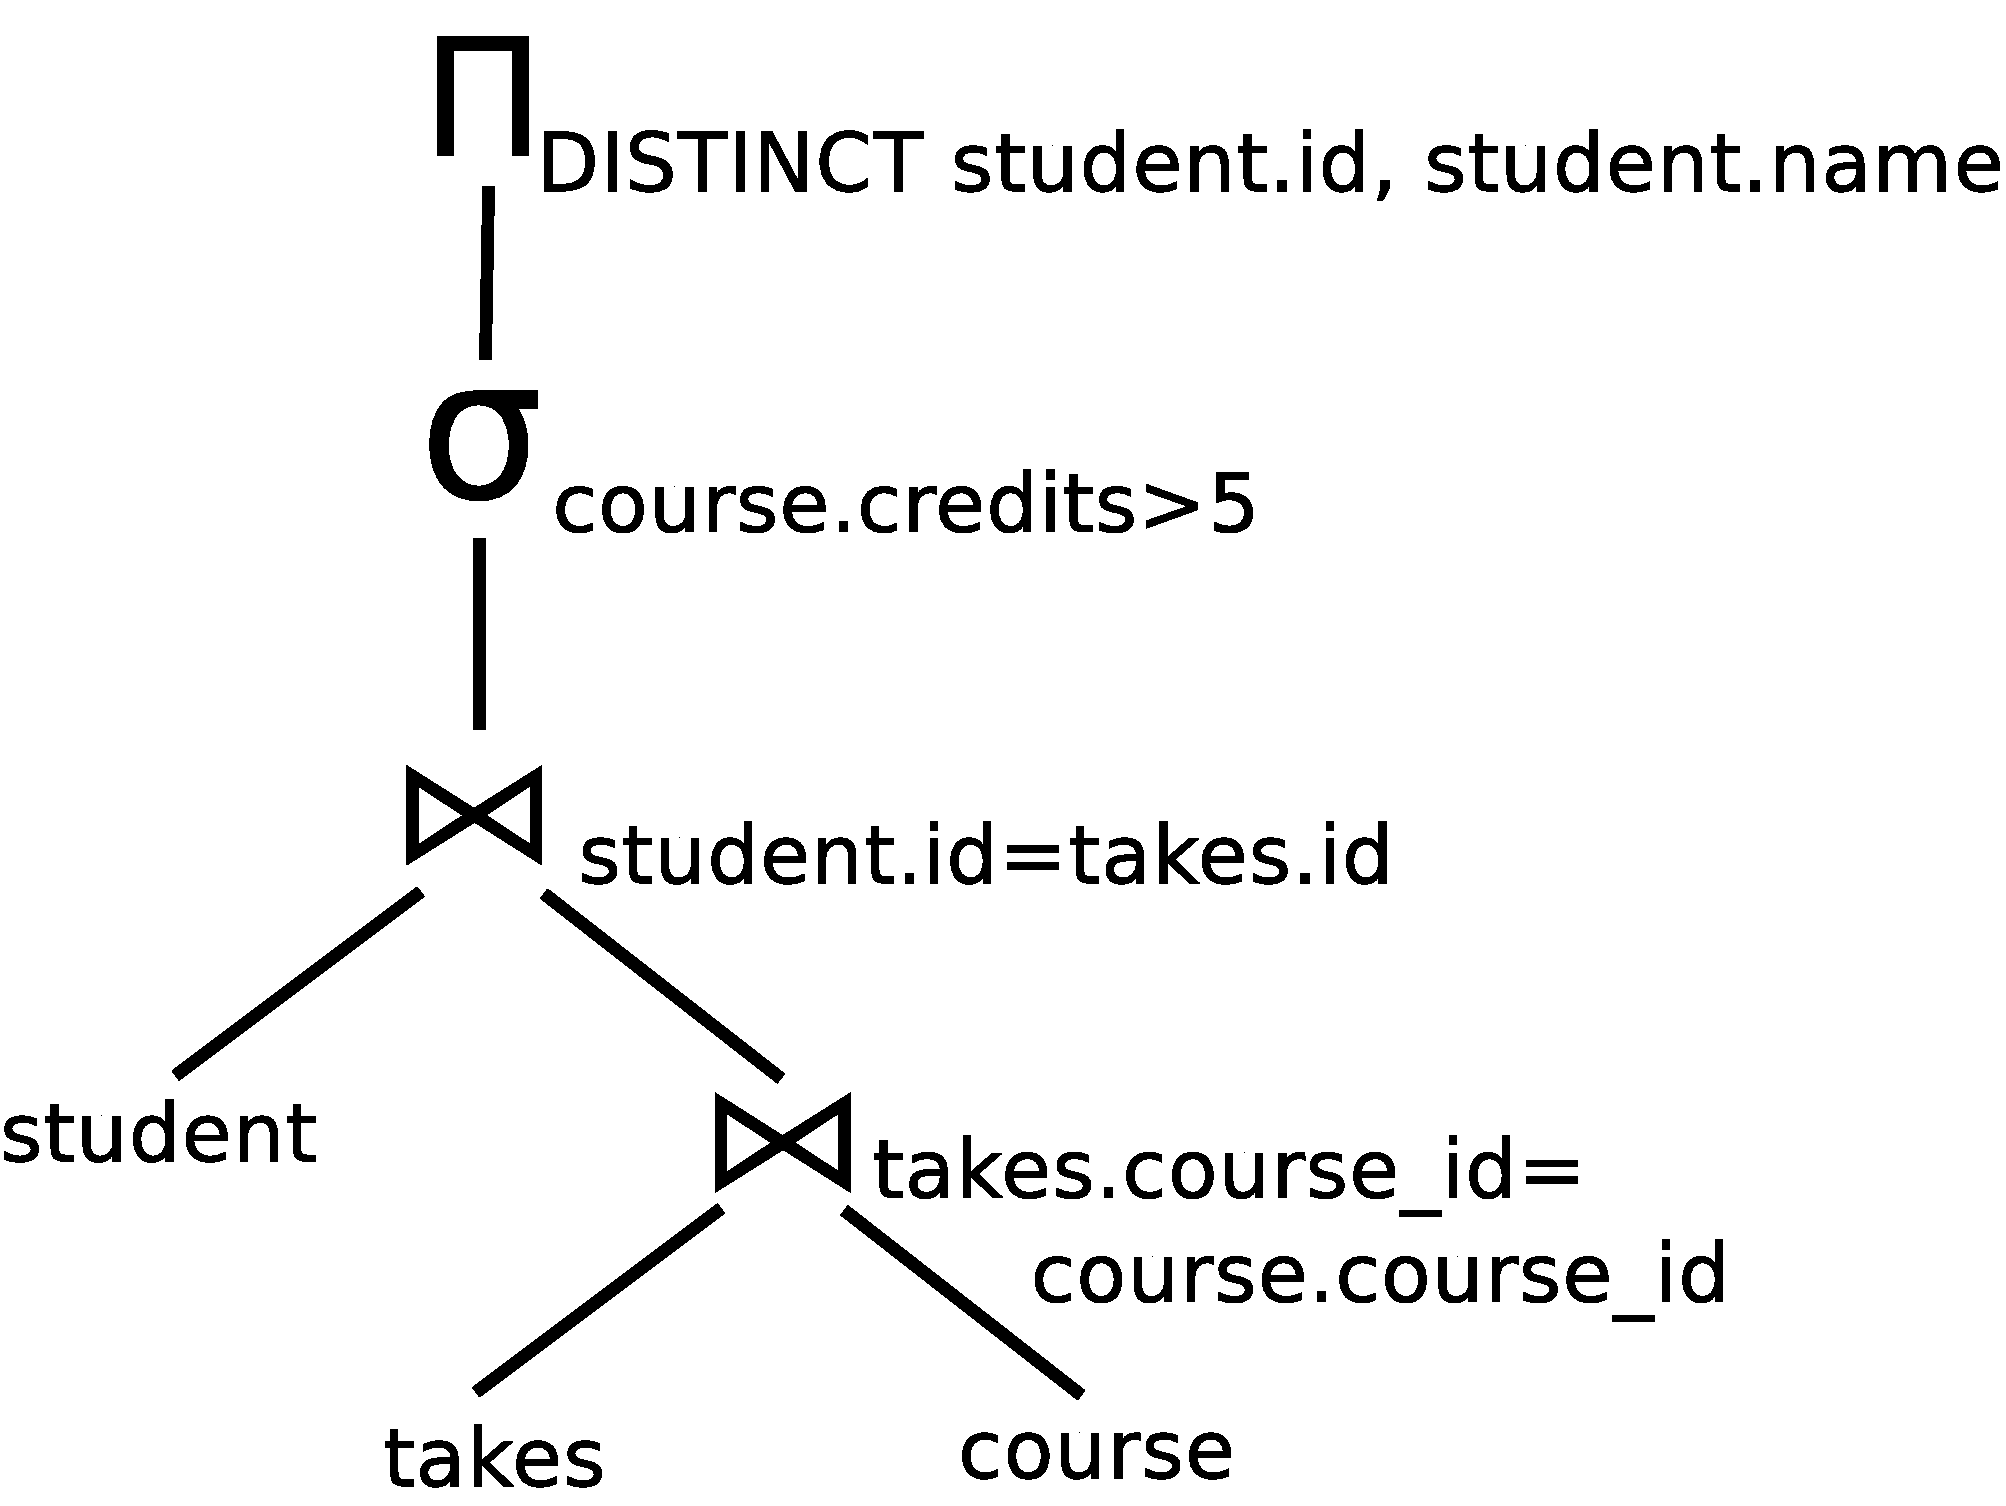
\includegraphics[width=1\textwidth,keepaspectratio=true]{/parsedTree.pdf}
		\caption{Parsed Tree From Query}
		\label{fig:parsedTree}
	\end{minipage}
		\begin{minipage}{0.59\textwidth}
	\centering
	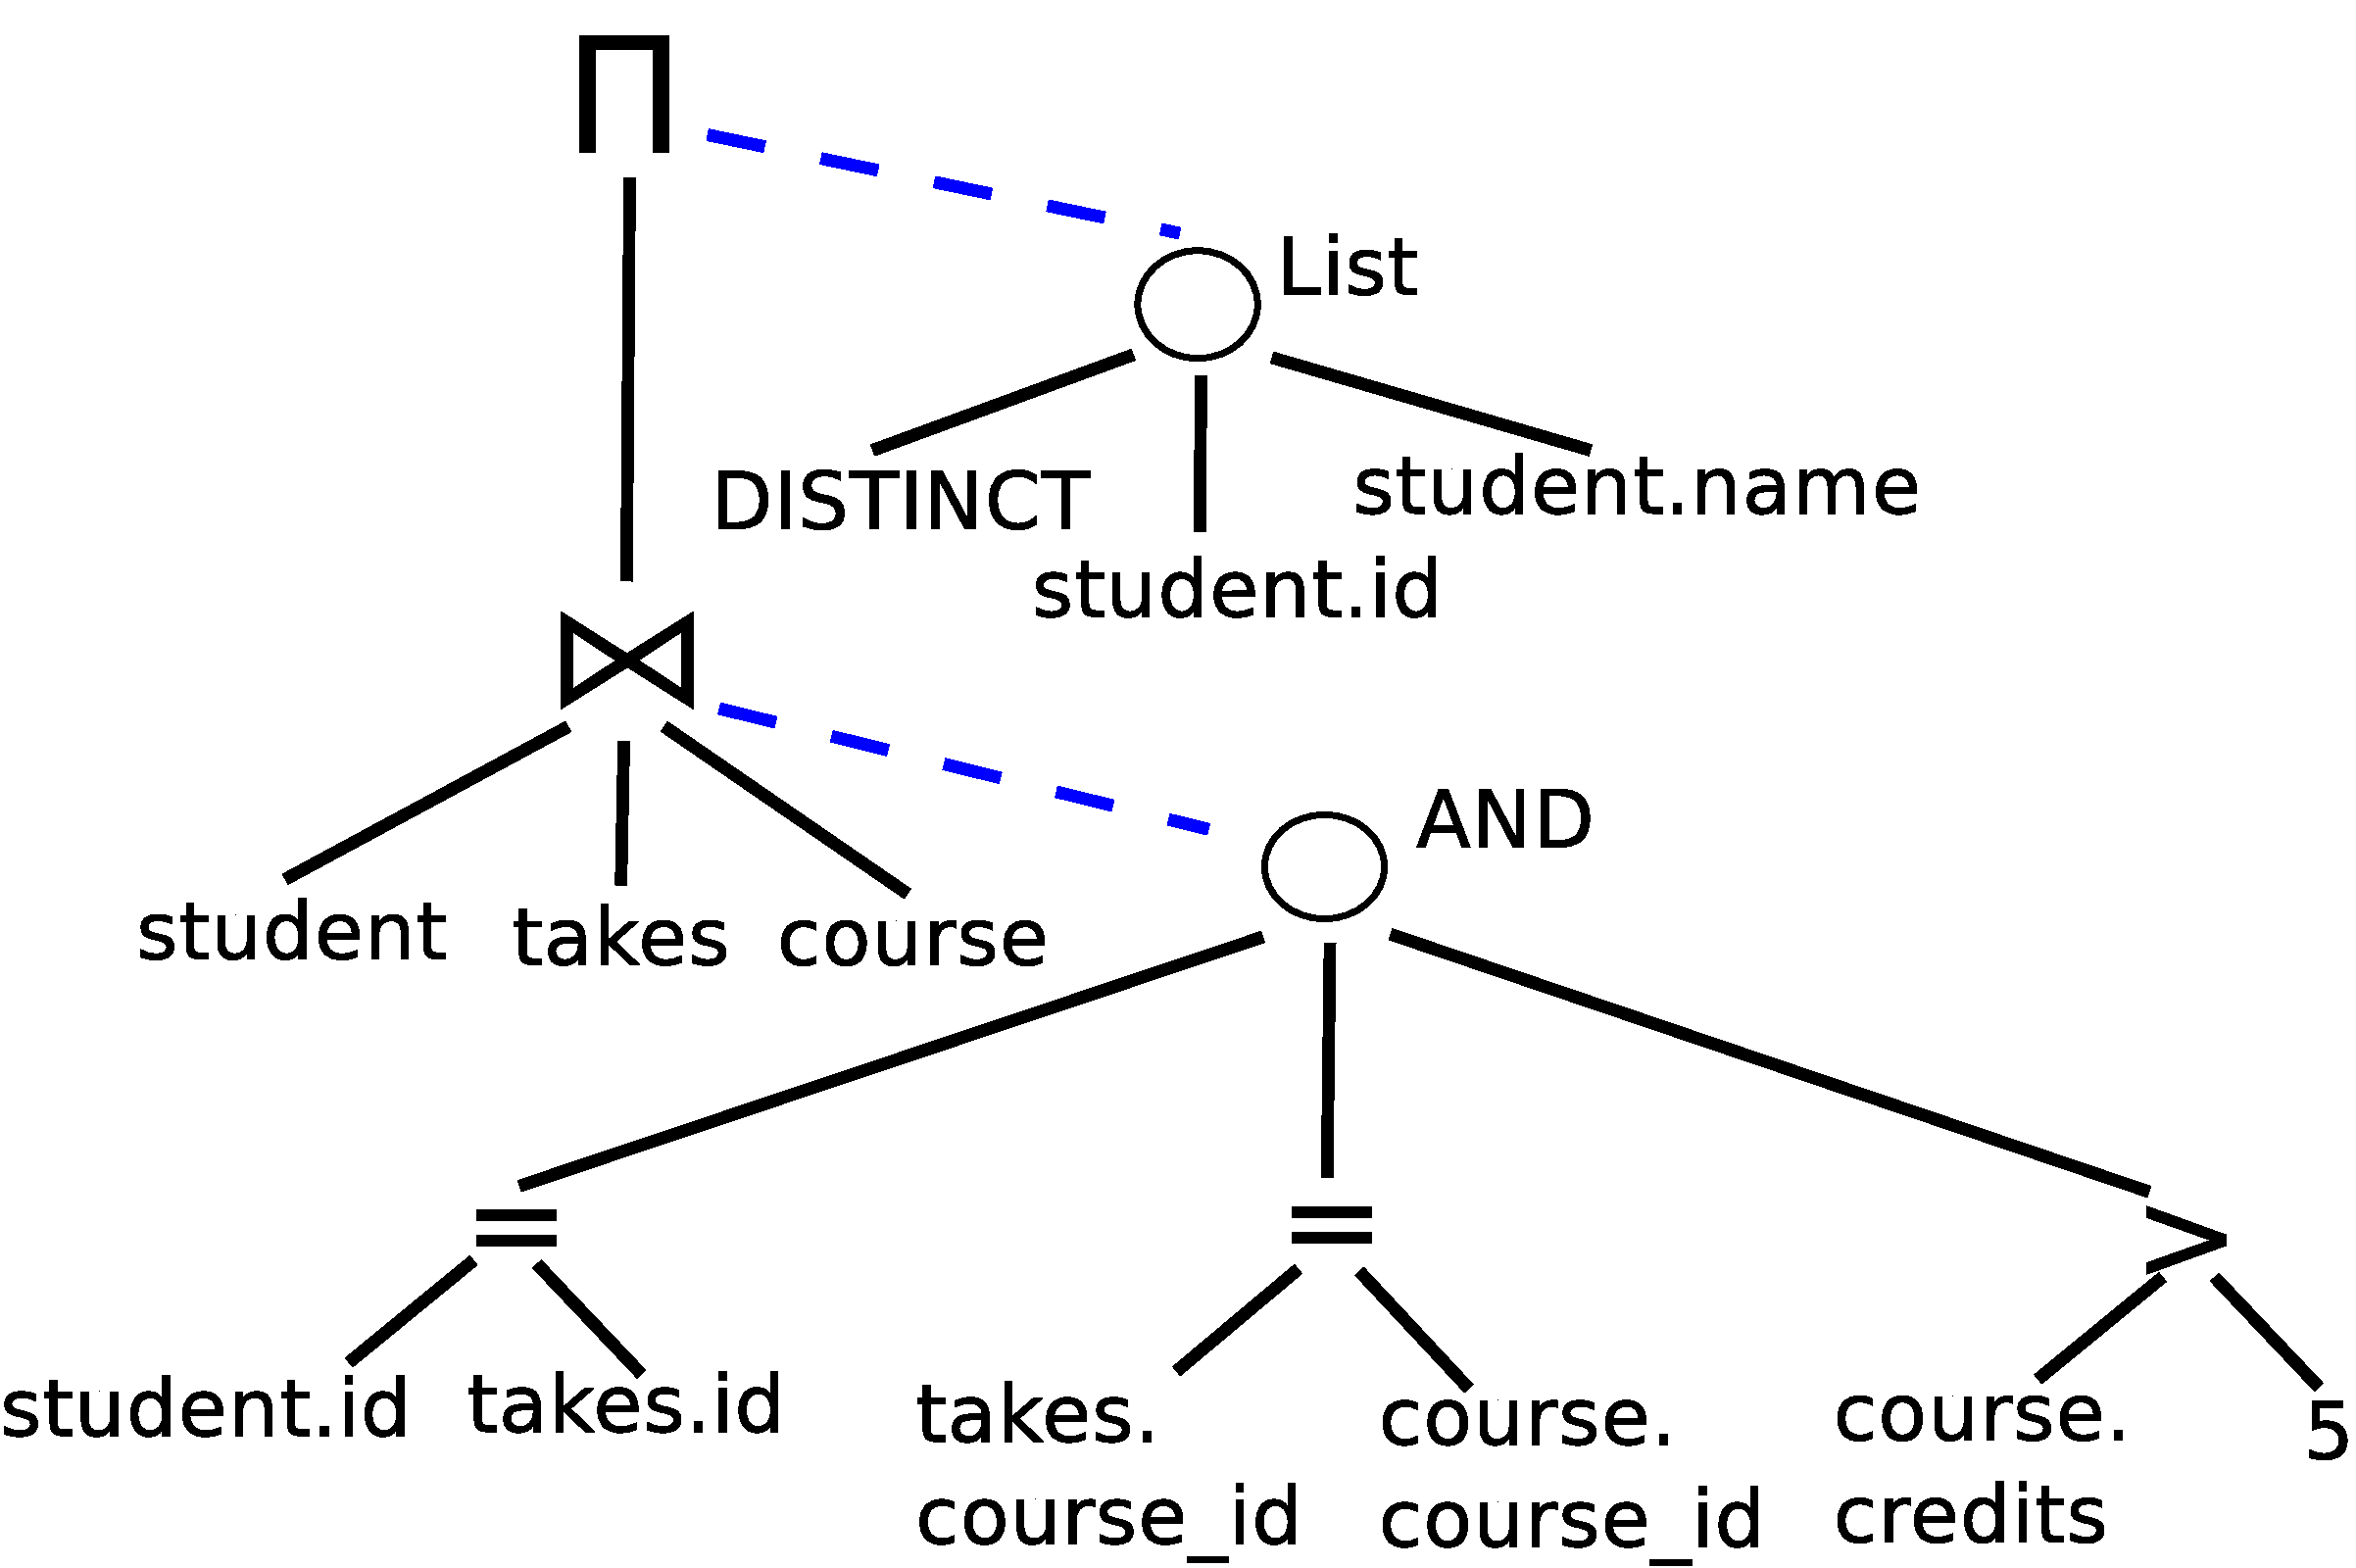
\includegraphics[width=1\textwidth,keepaspectratio=true]{/flattenedTree.pdf}
		\caption{Flattened Tree}
		\label{fig:flattenedTree}
	\end{minipage}
\end{figure}


\subsection{Edit Sequence Based Grading}
XData considers the following form of edits to the flattened tree generated from the student query.
\begin{itemize}
    \item  inserting a node/subtree into the flattened tree
\item removing a node/subtree from the flattened tree
\item replacing an existing node/subtree from a flattened tree
with another node/subtree in the flattened tree
\item moving a node/subtree from one position of the flattened
tree to another
\end{itemize}

When editing a flattened tree generated from a student query, an infinite number of possible edits could be made. However only edits that make the query more similar to the correct query would be useful. In order to add edits that make the student query more similar to the correct query, XData uses the correct query to guide the edits that are generated. The guided edits are based on the differences the student flattened student query tree has with the flattened tree of the correct query. For example, query attributes/conditions/constructs not used in the correct query but present in the student query will be removed when generating edits. 
For each query edit that XData generates, marks corresponding to the edit as configured by the instructor are deducted. The marks deducted for the edit can be considered the edit cost. 

XData can generate multiple guided edits on the student query at each step. From each of these edited queries, more edits are possible. Consider a graph whose nodes are all queries for the given schema. For a student query  SQ, edits of the query are also nodes in the graph. Let these edited queries be connected to query SQ with an edge whose weight is the edit cost of the edited query. Canonically equivalent queries, i.e. their canonical forms are the same, are connected by 0 cost edges. The sequence of edits that has the least cumulative cost can now be determined based on the shortest path in this graph from the student query node in the graph to a correct query node. Partial marks can now be awarded based on this shortest path.  Since the weight of each edge, which represents the cost of edit is non-negative, the shortest possible path may be found using Dijkstra’s shortest path algorithm. Hence, given a set of edits and using a given set of canonicalizations, the shortest path in the graph, as defined above, gives the edit sequence with the least cost.  
We note that the graph discussed above is for the ease of understanding only and XData does not proactively try to generate the entire graph. In practice, XData generates the nodes of the graph on the fly as needed. 

In case the instructor specifies multiple correct queries, the edit sequence based algorithm run based on all correct queries and the best partial marks obtained is awarded. 

\subsection{Heuristic solution}
Even with using only guided edits, the search space is still very large for larger queries if we consider all guided edits to get the shortest path from the student query to the correct query. Hence in practice, we use a greedy heuristic. The heuristic uses a cost benefit model. For each  edited query we can get an estimate of how incorrect the query is by finding the differences between the canonicalized versions of the edited query and the correct query. A weighted sum (based on the weight assigned by the instructor for each edit) can be used to find an edit distance which we call the \textit{canonicalized edit distance}. Each guided edit reduces the canonicalized edit distance to the correct query. The reduction in the canonicalized edit distance from the edit is the benefit of the edit. 

For the heuristic algorithm, at each edit step, we find the $benefit-cost$ for each edit. We then pick the edit that has the highest value of the $benefit-cost$ and use it to generate further edits. The remaining edits are discarded at each step. Using the heuristic allows XData to search a much smaller search space. For the incorrect student queries that we had in our course, we found that the heuristic solution works as well and takes orders of magnitude less time as compared to the exhaustive solution  \cite{xdata:comad}.



\section{Automated Grading Experience}
\label{sec:exp}
We have successfully used the XData automated grading system across several offerings of undergraduate database courses at IIT Bombay. Before using XData in a course, we empirically confirmed, using results from a previous database course, that XData was able to catch as many as or more errors than when the grading was done manually or when fixed datasets are used for grading. This result was consistent across all questions that XData was able to grade. We found, in several cases, that manual grading had missed subtle errors such as a missing distinct clause. 

For the initial course offerings, we used only generated dataset based grading to check for correctness and had to award partial marks manually. The dataset-based grading significantly reduced the human effort involved and allowed us to catch more errors than would have been possible with manual grading.
In several cases, however, students were not satisfied since they could not intuitively understand how marks had been deducted or what the error in their specific query was. The tagged datasets on which the student queries failed were shown but often there would be too many of them to understand the specific error. A dataset designed to catch one type of mutation may catch other types of mutations as well and hence it was not always clear what the actual error was. Several students contested the scores that they had been awarded when their query was found to be incorrect. Awarding partial marks manually by the graders was still tedious since students often wrote queries in very different and complex ways. Manually transforming such student queries to a simpler form was difficult. For instance, in one case a correct query involved using a NOT IN clause and some students used a combination of multiple EXCEPT and INTERSECT clauses.  

When using partial marking in combination with dataset based evaluation, we reduced the human effort as well as provided much better feedback. 
We experienced fewer students contest grades when it was assigned automatically compared to when a human would manually assign grades. The edit-based guidance was also  useful for students to understand where they went wrong. For the first course setting where we used automated partial marking for evaluation, we found that across 1800 student query submissions that were graded by XData, only 2 queries were contested by students. In both cases, we traced back the errors in grade to bugs in our code. One of the main challenges when using automated grading was to provide sufficient types of correct queries that covered the student queries.  

Since the edit sequence based guided edits provide a way to change an incorrect student query to a correct query, the guided edits can be used by students to learn the mistakes that they made and how the mistakes could have been corrected. Such feedback was very helpful especially for beginners to understand how to write correct SQL queries.  
\section{Related Work}
\label{sec:relwork}
There has been a significant interest in testing query equivalence or correctness and in automated grading. Related work include the following.

\subsection*{Checking Query Equivalence}

XData uses test data generation based on mutation testing to generate test datasets to check the equivalence of the correct query and student query. Tuya et al.~\cite{mutation1} describe a number of possible mutations for SQL queries. However, they do not handle test data generation for killing these mutations. Other approaches on testing query equivalence using datasets include Qex~\cite{QEX} and SQL full predicate coverage by Riva et al.~\cite{Riva:2010}. Test data generation in these systems is aimed at testing SQL queries in database applications and they consider only a limited subset of SQL query constructs. 

Techniques based on tableau~\cite{tableaux} and its extensions~\cite{tableaux1, tableaux2} can be used to check for query equivalence for a restricted class of conjunctive queries. Cosette~\cite{cosette} and U-semiring~\cite{semantic} can also be used to check for SQL semantic equivalence using a restricted set of axioms. 
SPES~\cite{spes} uses a symbolic approach for checking query equivalence on SQL queries under bag semantics for select-project-join(SPJ) queries as well as aggregate and union queries. 

\subsection*{Grading SQL Queries}
The Gradiance system~\cite{gradience} provides multiple choice type questions where the instructor has to provide some correct as well as incorrect answers and explanations of incorrectness. In such assignment settings, since the students are only able to select from limited options, subtle mistakes that students could make may not always be covered by the incorrect answers. Gradescope\cite{gradescope}, uses a fixed dataset to evaluate the correctness of student SQL queries. As discussed earlier, using fixed datasets may miss errors and would not be able to provide any meaningful feedback to incorrect student queries. RATest~\cite{rattest} provides feedback for incorrect queries by deriving small datasets that produce different results in a student query as compared to a correct query. I-Rex~\cite{irex} allows users to trace the SQL query evaluation for each constituent block in the query execution. 


\subsection*{Automated Grading for Programming Assignments}
Grading programming assignments has some similar challenges as grading database queries. CPSGrader~\cite{cpsgrader} can grade programming assignments for cyber-physical systems using constraints synthesis and uses reference solutions to provide feedback. AutoGrader~\cite{autograder} can grade introductory level python programs and provide student feedback using program synthesis and high-level error modeling specifications. However, AutoGrader can only model specific predictable errors. 

SARFGEN~\cite{sarfgen} provides feedback to student queries by aligning student programs to similar correct reference programs and finds the minimum number of edits to the student program to match the chosen reference program.  This approach is similar to our approach of edit-based grading. However, SQL queries have database constraints that are not part of the query but need to be accounted for during edits and equivalence checking. Hence we have a more complex semantic canonicalization step that can take into account constraints such as primary keys and foreign keys.





%%%%%%%%%%%%%%%%%%%%%%%%%%%%%%%%%%%%%%%%%
\section{Conclusion and Open Challenges}
\label{sec:conclusion}
The XData system is very useful for grading assignments on SQL queries and for providing feedback to students about mistakes they made. For large classes or online courses, such automated grading systems are essential and the automated individualized feedback would be very useful to new learners. Our experience in using the grading system has been very positive from both the teaching assistants as well as the students. The XData grading system as well as the  source code
are available for download from {\url{http://www.cse.iitb.ac.in/infolab/xdata}}.


One of the key challenges in the XData grading scheme is the number of ways a correct SQL query can be written. We have found that students sometimes write queries using a very different approach than we had anticipated. Catching errors with such approaches as well as awarding partial marks in these cases may be challenging. One way to address these would be to automatically group student query submissions and generate datasets for one student query in each group. We could then use the datasets to identify correct queries from the group and automatically add these as additional correct queries for grading. 
Another key challenge is in dealing with student queries that have additional query constructs that do not affect the query results. One of the cases that we found in our course was when a student had used the query {\smalltt{Q UNION Q'}} where Q' was always empty. The query had one error in Q but marks were also deducted based on edit for Q'.  


\paragraph*{Acknowledgments:} We thank all students and researchers who worked on the XData project as well as those who used the system and provided their valuable feedback. This work was partially supported by research funding and a PhD fellowship from Tata Consultancy Services. 
%%%%%%%%%%%%%%%%%%%%%%%%%%%%%%%%%%%%%%
%\bibliographystyle{IEEEtran}
%\bibliography{references}

\documentclass[11pt]{article}
%\documentclass[11pt,dvipdfm]{article}

\usepackage{deauthor}
\usepackage{url}            % simple URL typesetting
\usepackage{graphicx}
\usepackage{times}
\usepackage{fancyvrb}
\usepackage{comment}

% \graphicspath{{authorname/}}

\begin{document}

%\title{MLflow: An Open Platform for Machine Learning Experimentation, Reproducibility and Production}
%\title{MLflow: An Open Platform for the End-to-End Machine Learning Lifecycle}
\title{Accelerating the Machine Learning Lifecycle with {MLflow}}

% The \author macro works with any number of authors. There are two
% commands used to separate the names and addresses of multiple
% authors: \And and \AND.
%
% Using \And between authors leaves it to LaTeX to determine where to
% break the lines. Using \AND forces a line break at that point. So,
% if LaTeX puts 3 of 4 authors names on the first line, and the last
% on the second line, try using \AND instead of \And before the third
% author name.

\author{
  \textbf{Matei Zaharia, Andrew Chen, Aaron Davidson, Ali Ghodsi, Sue Ann Hong, Andy Konwinski,}\\
  \textbf{Siddharth Murching, Tomas Nykodym, Paul Ogilvie, Mani Parkhe, Fen Xie, Corey Zumar} \\
  Databricks Inc.\\
  %% examples of more authors
  %% \And
  %% Coauthor \\
  %% Affiliation \\
  %% Address \\
  %% \texttt{email} \\
  %% \AND
  %% Coauthor \\
  %% Affiliation \\
  %% Address \\
  %% \texttt{email} \\
  %% \And
  %% Coauthor \\
  %% Affiliation \\
  %% Address \\
  %% \texttt{email} \\
  %% \And
  %% Coauthor \\
  %% Affiliation \\
  %% Address \\
  %% \texttt{email} \\
}

\maketitle

\begin{abstract}
Machine learning development creates multiple new challenges that are not present in a traditional software development lifecycle.
These include keeping track of the myriad inputs to an ML application (e.g., data versions, code and tuning parameters), reproducing results, and production deployment.
In this paper, we summarize these challenges from our experience with Databricks customers, and describe MLflow, an open source platform we recently launched to streamline the machine learning lifecycle.
MLflow covers three key challenges: experimentation, reproducibility, and model deployment, using generic APIs that work with any ML library, algorithm and programming language.
The project has a rapidly growing open source community, with over 50 contributors since its launch in June 2018.
\end{abstract}

\section{Introduction}

Machine learning development requires solving new problems that are not part of the standard software development lifecycle.
For example, while traditional software has a well-defined set of product features to be built, ML development tends to revolve around \emph{experimentation}: the ML developer will constantly experiment with new datasets, models, software libraries, tuning parameters, etc.~to optimize a business metric such as model accuracy.
Because model performance depends heavily on the input data and training process, \emph{reproducibility} is paramount throughout ML development.
Finally, in order to have business impact, ML applications need to be \emph{deployed} to production, which means both deploying a model in a way that can be used for inference (e.g., REST serving) and deploying scheduled jobs to regularly update the model.
This is especially challenging when deployment requires collaboration with another team, such as application engineers who are not ML experts.

Based on our conversations with dozens of Databricks customers that use machine learning, these lifecycle problems are a major bottleneck in practice.
Although today's ML libraries provide tools for part of the lifecycle, there are no standard systems and interfaces to manage the full process.
For example, TensorFlow offers a training API and a Serving system~\cite{tfx}, but TensorFlow Serving cannot easily be used for models from another ML library, or from an incompatible version of TensorFlow.
In practice, an organization will need to run models from multiple ML libraries, TensorFlow versions, etc., and has to design its own infrastructure for this task.


Faced with these challenges, many organizations try to ``lock down'' the ML development process to obtain reproducibility and deployability.
Some organizations develop internal guidelines for ML development, such as which libraries one can use that the production team will support.
Others develop internal \emph{ML platforms} (e.g., Facebook's FBLearner~\cite{fblearner}, Uber's Michelangelo~\cite{michelangelo} and Google's TFX~\cite{tfx}): APIs that ML developers must use in order to build deployable models.
Unfortunately, both approaches limit ML developers in the algorithms and libraries they can use, decreasing their ability to experiment, and both create substantial engineering work whenever the ML developers want to use new libraries or models.

%Some organizations ask each ML team to manage its own infrastructure, which is expensive.
%Others try to develop shared \emph{ML platforms} that data scientists must use to build their models (e.g., Facebook's FBLearner~\cite{fblearner} and Uber's Michelangelo~\cite{michelangelo}), but this approach also has challenges, because model developers are limited to the algorithms and libraries supported by the platform and cannot easily experiment with others.

In this paper, we summarize our experience with ML lifecycle challenges at Databricks customers and describe MLflow, an open source ML platform we are developing to address these challenges.
MLflow's key principle is an \emph{open interface} design, where data scientists and engineers can bring their own training code, metrics, and inference logic while benefitting from a structured development process.
%MLflow leverages simple, generic interfaces such as Docker containers and REST APIs to achieve this goal.
For example, a ``model'' saved in MLflow can simply be a Python function (and associated library dependencies) that MLflow then knows how to deploy in various environments (e.g., batch or real-time scoring).
Other MLflow abstractions are likewise based on generic interfaces, such as REST APIs and Docker containers.
Compared to existing ML platforms like FBLearner, Michelangelo and TFX, this open interface design gives users flexibility and control while retaining the benefits of lifecycle management.
%Moreover, MLflow's open source nature enables easily sharing ML work across organizations.
The current version of MLflow provides APIs for experiment tracking, reproducible runs and model packaging and deployment, usable in Python, Java and R.
We describe these APIs and some sample MLflow use cases to show how the system can streamline the machine learning lifecycle.

\section{Challenges in Machine Learning Development}

ML faces many of the challenges in traditional software development, such as testing, code review, monitoring, etc.
In other ways, however, ML applications are different from traditional software, and present new problems.

One of the main differences is that the goal in machine learning is to \emph{optimize} a specific metric, such as prediction accuracy, instead of simply meeting a set of functional requirements.
For example, for a retailer, every 1\% improvement in prediction accuracy for a recommendation engine might lead to millions of dollars in revenue, so the ML team working on this engine will continuously want to improve the model.
This means that ML developers wish to continuously experiment with the latest models, software libraries, etc.,~to improve target metrics.
Beyond this difference in objective, ML applications are more complex to manage because their performance depends on training data, tuning, and concerns such as overfitting that do not occur in other applications.
%This means that reproducibility of these runtime conditions is important.
Finally, ML applications are often developed by teams or individuals with very different expertise, and hand-off between these individuals can be challenging.
For example, a data scientist might be an expert at ML training, and use her skills to create a model, but she might need to pass the model to a software engineer for deployment within an application.
Any errors in this process (e.g., mismatched software versions or data formats) might lead to incorrect results that are hard for a software engineer without ML knowledge to debug.

Based on these requirements in working with ML, we found four challenges to arise repeatedly at ML users:

\vspace{-0.6em}
\paragraph{1. Multitude of tools.} Hundreds of software tools cover each phase of ML development, from data preparation to model training to deployment. However, unlike traditional software development, where teams select \emph{one} tool for each phase, ML developers usually want to try \emph{every} available tool (e.g., algorithm) to see whether it improves results. For example, a team might try multiple preprocessing libraries (e.g., Pandas and Apache Spark) to featurize data; multiple model types (e.g. trees and deep learning); and even multiple frameworks for the same model type (e.g., TensorFlow and PyTorch) to run various models published online by researchers. %This diversity of tools means that ML teams need to use and productionize dozens of libraries.

\vspace{-0.6em}
\paragraph{2. Experiment tracking.} Machine learning results are affected by dozens of configurable parameters, ranging from the input data to hyperparameters and preprocessing code. Whether an individual is working alone or on a team, it is difficult to track which parameters, code, and data went into each experiment to produce a model.

\vspace{-0.6em}
\paragraph{3. Reproducibility.} Without detailed tracking, teams often have trouble getting the same code to work again. For example, a data scientist passing her training code to an engineer for use in production might see problems if the engineer modifies it, and even a user working alone needs to reliably reproduce old results to stay productive. %Even ML researchers frequently experience this problem when trying to reproduce published work.

\vspace{-0.6em}
\paragraph{4. Production deployment.} Moving an application to production can be challenging, both for inference and training. First, there are a plethora of possible inference environments, such as REST serving, batch scoring and mobile applications, but there is no standard way to move models from any library to these diverse environments. Second, the model training pipeline also needs to be reliably converted to a scheduled job, which requires care to reproduce the software environments, parameters, etc.~used in development.
Production deployment is especially challenging because it often requires passing the ML application to a different team with less ML expertise.

~

\vspace{-0.6em}
To address these problems, we believe that ML development processes should be explicitly designed to promote reproducibility, deployability, etc. The challenge is how to do so while leaving maximum flexibility for ML developers to build the best possible model. This led us to the open interface design philosophy for MLflow.

\section{MLflow Overview}

To structure the ML development process while leaving users maximum flexibility, we built MLflow around an \emph{open interface} philosophy: the system should define general interfaces for each abstraction (e.g., a training step, a deployment tool or a model) that allow users to bring their own code or workflows.
For example, many existing ML tools represent models using a serialization format, such as TensorFlow graphs~\cite{abadi2016tensorflow}, ONNX~\cite{onnx} or PMML~\cite{pmml}, when passing them from training to serving. This restricts applications to using specific libraries.
In contrast, in MLflow, a model can be represented simply as a Python function (and library dependency information), so any development tool that knows how to run a Python function can run such a model.
For more specialized deployment tools, a model can also expose other interfaces called ``flavors" (e.g., an ONNX graph) while still remaining viewable as just a Python function.
As another example, MLflow exposes most of its features through REST APIs that can called from any programming language.

More specifically, MLflow provides three components, which can either be used together or separately:

\begin{itemize}
\item \textbf{MLflow Tracking}, which is an API for recording experiment runs, including code used, parameters, input data, metrics, and arbitrary output files. These runs can then be queried through an API or UI.

\item\textbf{MLflow Projects}, a simple format for packaging code into reusable projects. Each project defines its environment (e.g., software libraries required), the code to run, and parameters that can be used to call the project programmatically in a multi-step workflow or in automated tools such as hyperparameter tuners.

\item\textbf{MLflow Models}, a generic format for packaging models (both the code and data required) that can work with diverse deployment tools (e.g., batch and real-time inference). %The goal is to give users of the model (e.g., a production engineer) a consistent interface for working with models built in different tools.
\end{itemize}

%We next sketch these components in turn; full documentation on them is available at \url{mlflow.org}.

\subsection{MLflow Tracking}

MLflow Tracking is an API for logging and querying \emph{experiment runs}, which consist of parameters, code versions, metrics and arbitrary output files called \emph{artifacts}. Users can start/end runs and log metrics, parameters and artifacts using simple API calls, as shown below using MLflow's Python API:

\begin{Verbatim}[frame=single,fontsize=\small,samepage=true]
# Log parameters, which are arbitrary key-value pairs
mlflow.log_param("num_dimensions", 8)
mlflow.log_param("regularization", 0.1)

# Log metrics; each metric can also be updated throughout the run
mlflow.log_metric("accuracy", 0.8)
mlflow.log_metric("r2", 0.4)

# Log artifacts (arbitrary output files)
mlflow.log_artifact("precision_recall.png")
\end{Verbatim}

MLflow Tracking API calls can be inserted anywhere users run code (e.g., standalone applications or Jupyter notebooks running in the cloud). The tracking API logs results to a local directory by default, but it can also be configured to log over the network to a server, allowing teams to share a centralized MLflow tracking server and compare results from multiple developers.

Once users have recorded runs, MLflow allows users to query them through an API or web-based UI (Figure~\ref{fig:tracking-ui}). This UI includes the ability to organize runs into groups called Experiments, search and sort them, and compare groups of runs, enabling users to build a custom leaderboard for each of their ML problems and even compare results across teams. The UI is inspired by experiment visualization tools such as Sacred~\cite{sacred}, ModelDB~\cite{modeldb} and TensorBoard~\cite{tensorboard}, and supports similar visualizations and queries.

\begin{figure}[h]
\centering
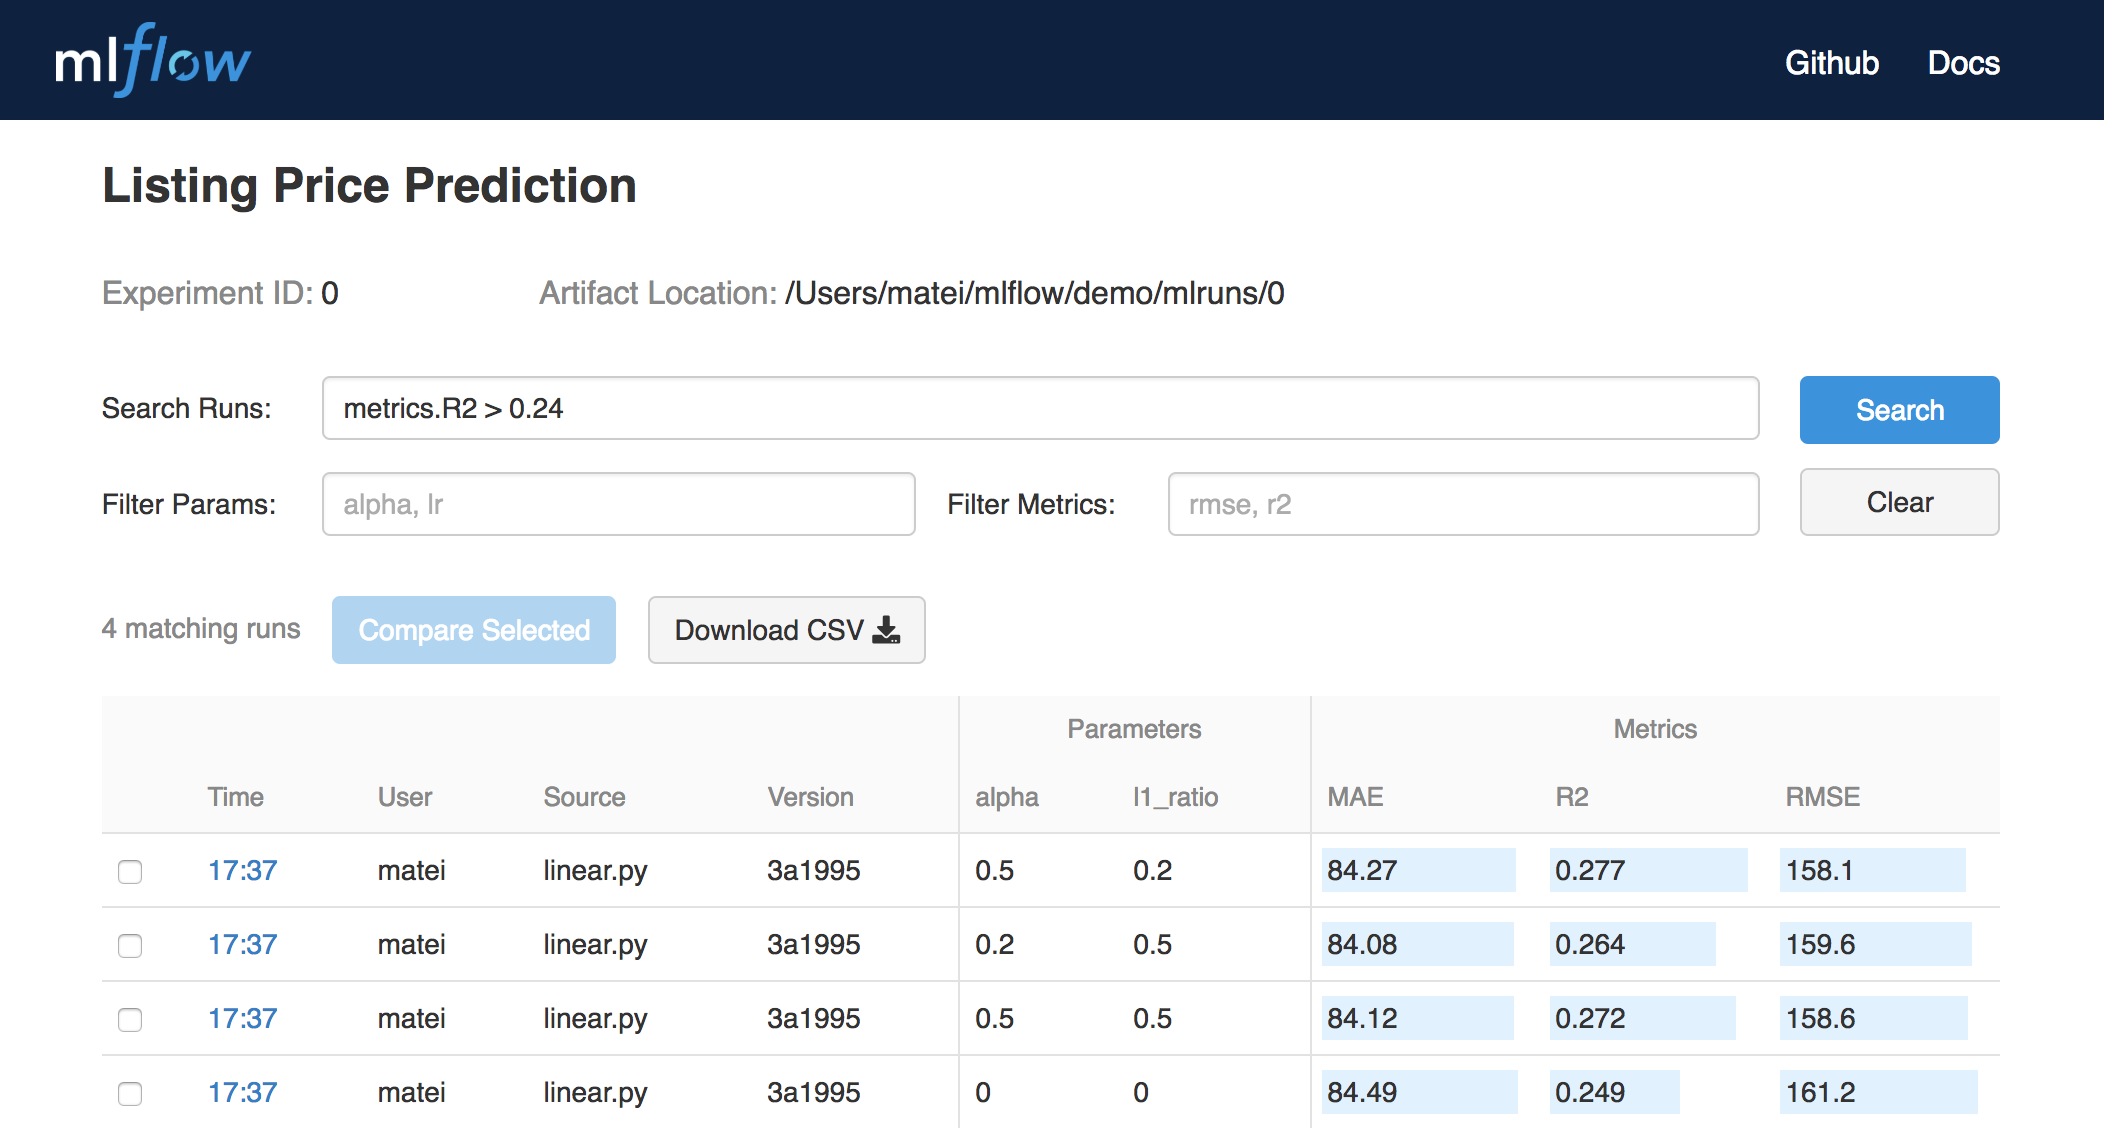
\includegraphics[bb=0 0 1052 564,width=\textwidth]{tracking.png}
\caption{MLflow Tracking UI showing several runs in an experiment. Clicking each run lists its metrics, artifacts and output details and lets the user post comments about the run.}
\label{fig:tracking-ui}
\end{figure}

\subsection{MLflow Projects}

MLflow Projects provide a simple format for packaging reproducible data science code. Each project is simply a directory with code or a Git repository, and uses a descriptor file to specify its dependencies and how to run the code. A MLflow Project is defined by a simple YAML file called MLproject, as shown below:

\begin{Verbatim}[frame=single,fontsize=\small,samepage=true]
name: My Project
conda_env: conda.yaml
entry_points:
  main:
    parameters:
      data_file: path
      alpha: {type: float, default: 0.1}
    command: "python train.py --reg-param {alpha} --data {data_file}"
\end{Verbatim}


Projects can specify their dependencies through a Conda environment or (in an upcoming release) a Docker container specification. A project may also have multiple entry points for invoking runs, with named parameters that downstream users can provide without understanding the internals of the project.

Users can run projects using the \texttt{mlflow run} command line tool, either from local files or a Git repository:

\begin{Verbatim}[frame=single,fontsize=\small,samepage=true]
mlflow run git@github.com:databricks/mlflow-example.git -P alpha=0.5
\end{Verbatim}

Alternatively, projects can be called programmatically using MLflow's API. This can be used to implement multi-step workflows or to pass projects a ``black box'' into automated tools such as hyperparameter search~\cite{hyperopt}.

In either case, MLflow will automatically set up the project's runtime environment and execute it. If the code inside the project uses the MLflow Tracking API, MLflow will also remember the project version executed (that is, the Git commit) and show an \texttt{mlflow run} command to re-execute it in its UI. Finally, MLflow projects can also be submitted to cloud platforms such as Databricks for remote execution.

\subsection{MLflow Models}

MLflow Models are a convention for packaging machine learning models in multiple formats called ``flavors'', allowing diverse tools to understand the model at different levels of abstractions. MLflow also offers a variety of built-in tools to deploy models in its standard favors. For example, the same model can be deployed as a Docker container for REST serving, as an Apache Spark user-defined function (UDF) for batch inference, or into cloud-managed serving platforms like Amazon SageMaker and Azure ML.

Each MLflow Model is simply stored as a directory containing arbitrary files and an MLmodel YAML file that lists the flavors it can be used in and additional metadata about how it was created:

\begin{Verbatim}[frame=single,fontsize=\small,samepage=true]
time_created: 2018-02-21T13:21:34.12
run_id: c4b65fc2c57f4b6d80c6e58a9dcb9f01
flavors:
  sklearn:
    sklearn_version: 0.19.1
    pickled_model: model.pkl
  python_function:
    loader_module: mlflow.sklearn
    pickled_model: model.pkl
\end{Verbatim}

In this example, the model can be used with tools that support either the \texttt{sklearn} or \texttt{python\_function} model flavors. For example, the MLflow SciKit-Learn library knows how to load a \texttt{sklearn} model as a SciKit-Learn Python object, but other deployment tools, such as running the model in a Docker HTTP server, only understand lower-level flavors like \texttt{python\_function}.
In addition, models logged using MLflow Tracking APIs will automatically include a reference to that run's unique ID, letting users discover how they were built.

\section{Example Use Cases}

In this section, we describe three sample MLflow use cases to highlight how users can leverage each component.

\vspace{-0.6em}
\paragraph{Experiment tracking.} A European energy company is using MLflow to track and update hundreds of energy grid models. This team's goal is to build a time series model for every major energy producer (e.g., power plant) and consumer (e.g., factory), monitor these using standard metrics, and combine the predictions to drive business processes such as pricing. Because a single team is responsible for hundreds of models, possibly using different ML libraries, it was important to have a standard development and tracking process. The team has standardized on using Jupyter notebooks for development, MLflow Tracking for metrics, and Databricks jobs for inference.

\vspace{-0.6em}
\paragraph{Reproducible projects.} An online marketplace is using MLflow Projects to package deep learning jobs using Keras and run them in the cloud. Each data scientist develops models locally on his or her laptop using a small dataset, checks them into a Git repository with an MLproject file, and submits remote runs of the project to GPU instances in the cloud for large-scale training or hyperparameter search. Using MLflow Projects makes it easy to create the same software environment in the cloud and share project code between different data scientists.

\vspace{-0.6em}
\paragraph{Model packaging.} The data science team at an e-commerce site is using MLflow Models to package recommendation models for use by application engineers. The technical challenge here was that the recommendation application includes both a standard, ``off-the-shelf'' recommendation model and custom business logic for pre- and post-processing. For example, the application might include custom code to make sure that the recommended items are diverse. This business logic needs to change in sync with the model, and the data science team wants to control both the business logic and the model, without having to submit a patch to the web application each time this logic has to change.
Moreover, the team wants to A/B test distinct models with distinct versions of the processing logic.
The solution was to package both the recommendation model and the custom logic using the \texttt{python\_function} flavor in an MLflow Model, which can then be deployed and tested as a single unit. %This allows production engineers to deploy the recommendation code as they please without the processing logic falling out of sync with the model.

\section{Related Work}

Many software systems aim to simplify ML development.
The closest to our work are the end-to-end ``ML platforms'' at large web companies.
For example, Facebook's FBLearner lets users write reusable workflow steps that run over data in Apache Hive~\cite{fblearner};
Uber's Michelangelo gives users a toolkit of algorithms to choose from that it can automatically train and deploy~\cite{michelangelo}; and Google's TFX provides data preparation and serving tools around TensorFlow~\cite{tfx}.
Anecdotally, these platforms greatly accelerate ML development, showing the benefits of standardizing the ML lifecycle.
However, they generally restrict users to a specific set of algorithms or libraries, so teams are on their own when they step outside these boundaries.
Our goal in MLflow is to let users easily bring their own tools and software in as many steps in the process as possible through our ``open interface'' design.
This includes custom training steps, inference code, and logged parameters and artifacts.

Other systems also tackle specific problems within the ML lifecycle. For example, Sacred~\cite{sacred}, ModelDB~\cite{modeldb} and TensorBoard~\cite{tensorboard} let users track experiments; PMML~\cite{pmml} and ONNX~\cite{onnx} are cross-library model serialization formats; Clipper~\cite{clipper} can deploy arbitrary models as Docker containers; and CDE~\cite{cde}, CodaLab~\cite{codalab}, Binder~\cite{binder} and Repo2Docker~\cite{repo2docker} enable reproducible software runs. MLflow combines these concepts with new ones, such as multi-flavor model packaging, into a unified system design and API.

\section{Conclusion}

For machine learning to have widespread commercial impact, organizations require the same kinds of reliable engineering processes around ML that exist in other engineering disciplines such as software development. In this paper, we have described some of the key challenges that differentiate ML development from traditional software development, such as experimentation, reproducibility, and reliable production deployment. We have also described MLflow, a software platform that can structure the machine learning lifecycle while giving users broad flexibility to use their own ML algorithms, software libraries and development processes.
MLflow is available as open source software at \url{https://www.mlflow.org}.


{\small

\begin{thebibliography}{10}

  \bibitem{abadi2016tensorflow}
  M.~Abadi, P.~Barham, J.~Chen, Z.~Chen, A.~Davis, J.~Dean, M.~Devin,
    S.~Ghemawat, G.~Irving, M.~Isard, et~al.
  \newblock {TensorFlow: A System for Large-Scale Machine Learning}.
  \newblock In {\em OSDI}, volume~16, pages 265--283, 2016.

  \bibitem{tfx}
  D.~Baylor, E.~Breck, H.-T. Cheng, N.~Fiedel, C.~Y. Foo, Z.~Haque, S.~Haykal,
    M.~Ispir, V.~Jain, L.~Koc, C.~Y. Koo, L.~Lew, C.~Mewald, A.~N. Modi,
    N.~Polyzotis, S.~Ramesh, S.~Roy, S.~E. Whang, M.~Wicke, J.~Wilkiewicz,
    X.~Zhang, and M.~Zinkevich.
  \newblock Tfx: A tensorflow-based production-scale machine learning platform.
  \newblock In {\em Proceedings of the 23rd ACM SIGKDD International Conference
    on Knowledge Discovery and Data Mining}, KDD '17, pages 1387--1395, New York,
    NY, USA, 2017. ACM.

  \bibitem{hyperopt}
  J.~Bergstra, B.~Komer, C.~Eliasmith, D.~Yamins, and D.~D. Cox.
  \newblock Hyperopt: a python library for model selection and hyperparameter
    optimization.
  \newblock {\em Computational Science and Discovery}, 8(1):014008, 2015.

  \bibitem{binder}
  {Binder}.
  \newblock \url{https://mybinder.org}, 2018.

  \bibitem{clipper}
  D.~Crankshaw, X.~Wang, G.~Zhou, M.~J. Franklin, J.~E. Gonzalez, and I.~Stoica.
  \newblock Clipper: A low-latency online prediction serving system.
  \newblock In {\em Proceedings of the 14th USENIX Conference on Networked
    Systems Design and Implementation}, NSDI'17, pages 613--627, Berkeley, CA,
    USA, 2017. USENIX Association.

  \bibitem{fblearner}
  J.~Dunn.
  \newblock Introducing {FBLearner Flow}: Facebook’s {AI} backbone.
  \newblock
    \url{https://code.fb.com/core-data/introducing-fblearner-flow-facebook-s-ai-backbone/}.

  \bibitem{repo2docker}
  J.~Forde, T.~Head, C.~Holdgraf, Y.~Panda, G.~Nalvarte, M.~Pacer, F.~Perez,
    B.~Ragan-Kelley, and E.~Sundell.
  \newblock Reproducible research environments with repo2docker.
  \newblock ICML, 07/2018 2018.

  \bibitem{tensorboard}
  Google.
  \newblock Tensorboard: Visualizing learning.
  \newblock \url{https://www.tensorflow.org/guide/summaries_and_tensorboard}.

  \bibitem{pmml}
  A.~Guazzelli, W.-C. Lin, and T.~Jena.
  \newblock {\em PMML in Action: Unleashing the Power of Open Standards for Data
    Mining and Predictive Analytics}.
  \newblock CreateSpace, Paramount, CA, 2nd edition, 2012.

  \bibitem{cde}
  P.~J. Guo.
  \newblock {CDE}: A tool for creating portable experimental software packages.
  \newblock {\em Computing in Science and Engineering}, 14(4):32--35, 2012.

  \bibitem{michelangelo}
  J.~Hermann and M.~D. Balso.
  \newblock Meet {Michelangelo}: Uber’s machine learning platform.
  \newblock \url{https://eng.uber.com/michelangelo/}.

  \bibitem{sacred}
  {K}laus {G}reff, {A}aron {K}lein, {M}artin {C}hovanec, {F}rank {H}utter, and
    {J}\"urgen {S}chmidhuber.
  \newblock {T}he {S}acred {I}nfrastructure for {C}omputational {R}esearch.
  \newblock In {K}aty {H}uff, {D}avid {L}ippa, {D}illon {N}iederhut, and
    M.~{P}acer, editors, {\em {P}roceedings of the 16th {P}ython in {S}cience
    {C}onference}, pages 49 -- 56, 2017.

  \bibitem{codalab}
  P.~Liang et~al.
  \newblock {CodaLab}.
  \newblock \url{https://worksheets.codalab.org}, 2018.

  \bibitem{onnx}
  {ONNX Group}.
  \newblock {ONNX}.
  \newblock \url{https://onnx.ai}.

  \bibitem{modeldb}
  M.~Vartak, H.~Subramanyam, W.-E. Lee, S.~Viswanathan, S.~Husnoo, S.~Madden, and
    M.~Zaharia.
  \newblock Modeldb: A system for machine learning model management.
  \newblock In {\em Proceedings of the Workshop on Human-In-the-Loop Data
    Analytics}, HILDA '16, pages 14:1--14:3, New York, NY, USA, 2016. ACM.

  \end{thebibliography}


}
%\bibliographystyle{abbrv}
%\bibliography{paper}

\end{document}


\end{document}
